\documentclass[autodetect-engine, dvipdfmx-if-dvi, ja=standard, 12pt]{bxjsbook}

\usepackage{graphicx}        %図を表示するのに必要
\usepackage{color}           %jpgなどを表示するのに必要
\usepackage{amsmath,amssymb} %数学記号を出すのに必要
\usepackage{setspace}
\usepackage{cases}
\usepackage{here}
\usepackage{fancyhdr}
\usepackage{ascmac}
% \usepackage{titlesec}

\parindent = 0pt  % 行頭の字下げをしない
\setstretch{1.3}  % 行間を広めにとる

% 各章,節などタイトルの大きさを変更
% \titleformat*{\section}{\Huge\bfseries}
% \titleformat*{\subsection}{\Large\bfseries}

% 式の番号を(senction_num.num)のようにする
\makeatletter
\@addtoreset{equation}{chapter}
\def\theequation{\thechapter.\arabic{equation}}
\makeatother

% 呼び出したページのページ番号を消す
\newcommand{\deletePageNum}{
    \thispagestyle{empty}
    \clearpage
    \addtocounter{page}{-1}
}


\begin{document}

\begin{center}
    {\Large 令和元年度 卒業研究論文} \\[3.5truecm]
    \huge MATLAB/Simulinkによる\\RADAR計測システムの開発\\
    \LARGE Development on RADAR measurement system\\using MATLAB/Simulink\\[4truecm]
    \Large 一関工業高等専門学校\\
    電気情報工学科 秋田研究室\\
    佐藤 凌雅\\
     \\
    \today
\end{center}
\newpage

\begin{abstract}

    {\Large \bf 概要\par}
    \vspace{3mm}
     本研究は,路面の段差検知システムの実現を目的としている.提案するシステムはRADARを用いて路面を常に監視し,車両前方に段差が存在する際には運転手に警告することが可能である.また,システム構築にはMATLAB/Simulinkを用いたモデルベース開発を採用し,ソフトウェア設計の効率向上を図った.なお,提案した手法の有効性をシミュレーションと実際の車両での実験を通して検証した.\par
    \vspace{1mm}
    {\bf キーワード:}
    RADAR,モデルベース開発\par
    \vspace{7mm}

    {\Large \bf Abstract\par}
    \vspace{3mm}
    This study aims to realize a road step detection system. The proposed system can always monitor the road surface with RADAR and warn the driver if there is a step in front of the vehicle. In addition, in order to improve the efficiency of software design, model-based development using MATLAB/Simulink was adopted for system construction. The effectiveness of the proposed method is verified through a simulation and experiment.\par
    \vspace{1mm}
    {\bf Keyword:}
    RADAR, Model-Based Development\par

\end{abstract}

\deletePageNum
\newpage
\newpage

% \maketitle
\pagestyle{fancy}

\section{前書き}
 車両制御技術は,情報処理の先端技術として急速に発展している.たとえば,急ブレーキ時にホイールロックを防止するアンチロックブレーキシステム(ABS),滑りやすい路面でタイヤがスリップするのを抑制する電子安定性制御(ESC)などがあげられる.また,各車輪の駆動力を独立して制御して車両の挙動を安定させるダイレクトヨーモーメント制御(DYC)と,駆動力を制御することで所望のスリップ率を維持するスリップ率制御など.このような制御技術の発展により,自動車はこれまで以上に安全かつ安定して走行することが可能になってきた.運転支援システムは,交通事故件数の削減に大きく貢献し,さらなる発展が期待されている.\\
 近年,交通事故を減らす技術として自律型緊急ブレーキシステム(AEBS)が注目されている.AEBSの概要:車両に搭載されたカメラやレーダーが他の車両や前方の歩行者などの障害物を検出した場合,相対位置と相対速度から衝突の危険性を判断する.すると,システムは車両を減速させる.自動車製造業者の調査によると,事故の合計数は,非装備車と比較して61%減少し,後端事故の数は84%減少した.それはAEBSの重要性と有用性を証明している.\\
 しかしながら,現在の商用車のAEBSは,歩行者の現在位置に基づいて衝突の危険性を検出しており,歩行者の動きを考慮していないという問題がある.歩行者や障害物が車両の前方に存在する場合,システムはそれに対処することができ,衝突事故を回避することが可能である.一方,歩行者が横から歩くと,衝突の瞬間まで歩行者が車両の前に位置していないため,現在のAEBSは機能しない可能性がある.歩行者と車両との衝突事故は道路を横断する間にしばしば起こるので,歩行者運動に対応するAEBSは交通事故を減らすための重要なシステムである.\\
 歩行者の動きに対応して,歩行者の将来の位置を予測し,それに応じて制動力を制御する必要がある.したがって,有限時間における車両の位置がシステムの指令値となるように,時間領域で車両を制御する必要がある.\\
 そこで,時間領域での制御器設計法としてモデル予測制御(MPC)が注目されている.MPCは制約条件付きリアルタイム最適制御と呼ぶことができ,将来のシステム挙動を予測し,評価関数を最小化するように現在の入力値を決定する.MPCは二次計画問題を解決する必要があり,計算負荷が大きいため,プロセス制御の分野のようにサンプリング時間の長いシステムで広く使用されている.しかし,近年,計算機の計算速度が向上してきており,サンプリング時間の短いシステムへの適用が可能になってきている.MPCのもう一つの問題は,開ループコントローラである.制御性能はモデル精度に大きく依存し,外乱の感度が高いという欠点がある.\\
 外乱抑制と目標値への追従性を両立させるためには,外乱を推定しフィードフォワード制御で補償する必要がある.外乱とは,転がり抵抗,空気抵抗,坂道走行時に発生する勾配抵抗などの走行抵抗のことである.しかしながら,駆動力制御に関するこれまでの研究のほとんどは,駆動抵抗が非常に小さいと仮定し無視している.サンプリング時間が短いシステムの場合,フィードバックループによる駆動抵抗の影響を少なくすることができる.しかしながら,MPCはPID制御等よりもサンプリング時間が長く,外乱の影響が顕著になる.さらに,外乱はMPCにおける予測に使用されるモデルの精度を低下させるので,自動車の予測された挙動は実際のものから逸脱する.これでは所望の結果が得られない.したがって,MPCを駆動力制御に適用するためには,駆動抵抗の推定と補償を考慮する必要がある.\\
 一般に,人間はさまざまな道路環境や歩行者に基づいて危険を予測しながら運転する.ここでは,人間などの危険性を予測しながら車両を制御することを目的としており,歩行者の動きに対応するためのAEBSの改良につながる.この目的を達成するために,歩行者の将来の位置を予測するためのアルゴリズムの構築と運転抵抗を補償することができる時間領域におけるコントローラの設計について述べる.\\
 本論文では,車両に搭載されたカメラなどのセンシング機器から得られる歩行者の位置情報を想定している.提案手法の概要は以下の通りである.まず,歩行者速度は,現在の歩行者の位置からカルマンフィルタによって推定される.将来の歩行者の予測位置は,一定期間の歩行者速度の値から予測される.衝突の可能性がある場合は,車両の予測位置と比較してMPCにより制動力の指令値を算出する. MPCはモデルの精度に依存するため,外乱とパラメータ誤差の影響を強く受けるという欠点がある.そこで,制御性能を向上させるために制動力のフィードバックループを導入し,外乱である駆動抵抗の推定量を提案システムに含める.システムのコントローラはMPCと制動力フィードバック制御のカスケードコントローラである.提案した方法を利用することにより,歩行者の将来の位置を予測し,衝突の危険性を検出することが可能である.さらに,駆動抵抗を補償して制動力を制御することで,外乱感度を低下させながらシステムの追従性を向上させることができる.\\
 この論文は以下のように構成されている. 2章では提案手法のモデル化について説明し,3章で制御系の設計について述べる.4章と5章ではそれぞれシミュレーションと実験について説明する.最後に,結論は6章に示す.\\

\section{モデリング}
\subsection{車体モデル}
 車両と歩行者との衝突はまっすぐな道路上で起こることがほとんどであり,モデルを単純化するために直線運動のみを考慮した車両の車体モデルを図1に示す.\\
\begin{figure}[t]
    \centering
    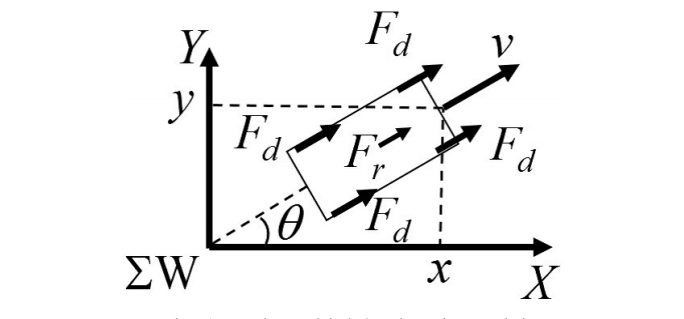
\includegraphics[width=8cm]{./fig/fig1.png}
    \caption{車両のシャシーモデル}
\end{figure}

 図1に示すように,車両の車体の運動学とダイナミクスは次のとおり.\\
\begin{flalign}
    &\dot{x} = v\cos(\theta)\\
    &\dot{y} = v\sin(\theta)\\
    &M\dot{v} = nF_d+F_r
\end{flalign}

 ここで $x$ と $y$ は車両の位置である. $v$,$\theta$,$M$,$n$,$F_d$,$F_r$ は,それぞれ車速,車両角度,車両質量,制御輪数,駆動力,駆動抵抗である.$\Sigma$ はワールド座標系を表す.したがって,$\Sigma$ の $x$ と $y$ は,それぞれ緯度と経度の位置を示す.一般的に,抵抗力は移動方向に対して反対方向を向いている.ただし,駆動抵抗は正の値でも負の値でも構わない.この論文では,$F_r$ は $F_d$ と同じ方向を向いている.\\
 ちなみに,本論文の制御法にはモデル予測制御(MPC)を含んでおり,MPCは離散状態で定式化される.したがって,車体モデルの線形移動のみを制限した離散時間状態空間表現は,次のように表される.\\
\begin{flalign}
    &{\boldsymbol x}[k+1] = {\boldsymbol Ax}[k]+B(u[k]+F_r) ,\\
    &{\boldsymbol z} = {\boldsymbol Cx}[k]
\end{flalign}
なお
\begin{flalign}
    &A = \left[
        \begin{array}{rrr}
            1 & 0 & T_s\cos\theta \\
            0 & 1 & T_s\sin\theta \\
            0 & 0 & 1
        \end{array}
    \right]\nonumber\\
    &B = \left[
        \begin{array}{rrr}
            \frac{1}{2M}T_s^2\cos\theta & \frac{1}{2M}T_s^2\sin\theta & \frac{T_s}{M}
        \end{array}
    \right]^{\mathrm{T}}\nonumber
\end{flalign}
 ここで $T_s$ はサンプリング時間を表している. $u[k]$ は各車輪の力の合計であり,システムの出力変数は状態変数に等しい. これは, $x$,$y$,$v$に関する情報を取得できることを示している.日本では準天頂衛星システム(QZSS)などの測位技術の開発により,車両の位置を高精度に計測できるため,論文はこれらの値が得られると仮定している.

\subsection{ホイールモデル}
図2に示すホイールモデルのダイナミクスは次のように説明される.
\begin{figure}[h]
    \centering
    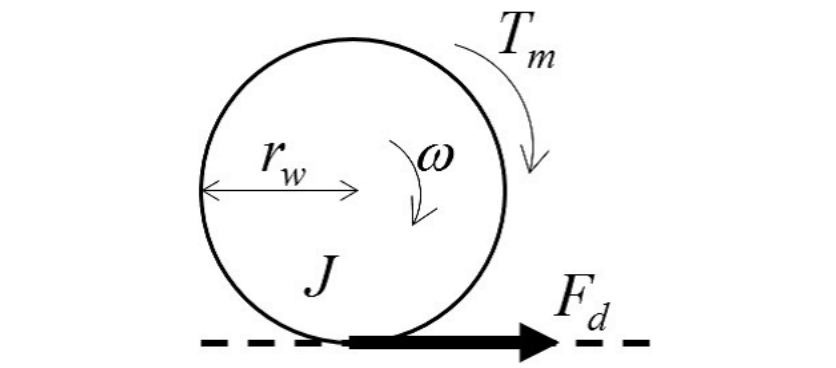
\includegraphics[width=8cm]{./fig/fig2.png}
    \caption{車両のホイールモデル}
\end{figure}

\begin{flalign}
    &J\dot{\omega} = T_m - r_m F_d\\
    &F_d = \mu(\lambda)\frac{Mg}{n}\\
    &\lambda = \frac{v-r_\omega\omega}{\mbox{max}(v,r_\omega\omega)}
\end{flalign}
ここで,$J$,$T_m$,$\omega$,$r_w$,$\lambda$および$\mu$は,それぞれモーターの慣性,モーターまたはブレーキ装置によって生成されるトルク,車輪角速度,車輪半径,スリップ率,および摩擦係数を表している. $\mu$はスリップ率$\lambda$の関数であり,$\mu$は法線力とタイヤ力の比を示していることに注意.

\subsection{摩擦円}
 摩擦円理論によれば,縦力Fxと横力Fyを含むタイヤ力は,式(9)となる.
\begin{equation}
    \sqrt{F^{x^{2}}+F^{y^{2}}} \leq \mu_{\max } M g
\end{equation}

 $\mu_{max}$は最大摩擦係数を示し,$g$は重力加速度である.式(9)は,縦力と横力の合力に上限があることを示している.合力が式の右側を超える場合,タイヤがスリップし,ドライバーが車両を制御できなくなる.したがって,スリップ現象を回避するためにはタイヤの力を制御する必要がある.

\section{制御システム設計}
 このセクションでは,2つのセクションで提案された制御システムについて説明する. 1つは衝突検出,もう1つはブレーキシステムである.

\subsection{衝突検出}
 歩行者と車両の衝突を検出するために,最初にカルマンフィルターを使用して歩行者の速度を推定する.状態空間表現と推定方程式は次のように説明される.
\begin{flalign}
    \boldsymbol{x}_{\boldsymbol{h}}[k+1]=& \boldsymbol{A}_{k} \boldsymbol{x}_{\boldsymbol{h}}[k]+\boldsymbol{G}_{k} \boldsymbol{\omega}, \\
    \boldsymbol{z}_{\boldsymbol{h}}[k]=& \boldsymbol{c}_{k} \boldsymbol{x}_{\boldsymbol{h}}[k]+\boldsymbol{J}_{k} \boldsymbol{v},\\
    \hat{\boldsymbol{x}}_{\boldsymbol{h}}[k]=& \boldsymbol{A}_{k} \hat{\boldsymbol{x}}_{\boldsymbol{h}}[k-1]\nonumber \\
    &+\boldsymbol{g}[k]\left(\boldsymbol{z}_{\boldsymbol{h}}[k]-\boldsymbol{c}_{\boldsymbol{k}} \boldsymbol{A}_{k} \hat{\boldsymbol{x}}_{h}[k-1]\right)
\end{flalign}

なお

\begin{flalign}
    \boldsymbol{A}_{k}&=\left[\begin{array}{llll}{1} & {0} & {T_{s}} & {0} \\ {0} & {1} & {0} & {T_{s}} \\ {0} & {0} & {1} & {0} \\ {0} & {0} & {1} & {0} \\ {0} & {0} & {0} & {1}\end{array}\right] \nonumber\\
    \boldsymbol{G}_{k}&=\left[\begin{array}{ccccc}{\frac{1}{2} T_{s}^{2}} & {0} & {T_{s}} & {0} \\ {0} & {\frac{1}{2} T_{s}^{2}} & {0} & {T_{s}}\end{array}\right]^{T} \nonumber\\
    \boldsymbol{c}_{k}&=\left[\begin{array}{cccc}{1} & {0} & {0} & {0} \\ {0} & {1} & {0} & {0}\end{array}\right] \nonumber\\
    \boldsymbol{J}_{k}&=\boldsymbol{I}_{2} \nonumber\\
    \boldsymbol{x}_{h}[k]&=\left[\begin{array}{ll}{x_{h}[k]} & {y_{h}[k]}\end{array} \quad \dot{x}_{h}[k] \quad y_{h}[k]\right]^{T} \nonumber\\
    \boldsymbol{z}_{h}[k]&=\left[\begin{array}{cc}{x_{h}[k]} & {y_{h}[k]}\end{array}\right]^{T} \nonumber
\end{flalign}

 ここで,$\omega$,$\nu$,および$g[k]$は,それぞれシステムノイズ,観測ノイズ,および最適なカルマンゲインを示すす.$\omega$,$\nu$はホワイトノイズである. $x_h$および$y_h$は,カメラデバイスまたは道路機器によって取得される歩行者の位置.カルマンフィルターを使用すると,歩行者の速度を推定できる.
 次に,有限時間における歩行者の位置が歩行者の速度から予測される.一定期間の歩行者の速度は2次正規分布に従うと想定される.これにより,確率密度関数が一定の場合,等確率楕円が作成される.等確率楕円の方程式は次のとおり.
\begin{flalign}
    &\frac{\left(\left(x-\mu_{x}\right) \cos \alpha+\left(y-\mu_{y}\right) \sin \alpha\right)^{2}}{\left(c \sigma_{u}\right)^{2}}\nonumber\\
    &+\frac{\left(-\left(x-\mu_{x}\right) \cos \alpha+\left(y-\mu_{y}\right) \sin \alpha\right)^{2}}{\left(c \sigma_{v}\right)^{2}} =1
\end{flalign}

なお

\begin{flalign}
    \sigma_{u}^{2} &=\frac{\sigma_{x}^{2}+\sigma_{y}^{2}+\sqrt{\left(\sigma_{x}^{2}-\sigma_{y}^{2}\right)+4 \sigma_{x y}^{2}}}{2} \nonumber\\
    \sigma_{v}^{2} &=\frac{\sigma_{x}^{2}+\sigma_{y}^{2}-\sqrt{\left(\sigma_{x}^{2}-\sigma_{y}^{2}\right)+4 \sigma_{x y}^{2}}}{2} \nonumber\\
    \alpha &=\arctan \frac{\sigma_{u}^{2}-\sigma_{x}^{2}}{\sigma_{x y}} \nonumber
\end{flalign}

 ここで,$\mu_x$と$\mu_y$は平均値,$\sigma_x$,$\sigma_y$は標準偏差,$\sigma_{xy}$は歩行者の速度の共分散である.さらに,$\alpha$は等確率楕円の角度を示す. $c$は確率密度関数$f$に依存し,$c$と$f$の関係を表1に示す.
\begin{table}[]
    \centering
    \caption{$f$と$c$の関係}
    \begin{tabular}{|l|l|}
    \hline
    f     & c      \\ \hline
    0.393 & 1.000  \\ \hline
    0.500 & 1.177  \\ \hline
    0.900 & 2.146 \\ \hline
    0.950 & 2.448 \\ \hline
    0.990 & 3.035  \\ \hline
    \end{tabular}
\end{table}
したがって,式(13)は1秒での歩行者の予測位置を示す.一方,入力なしの車両の予測位置は次のように定式化される.
\begin{flalign}
    \hat{\boldsymbol{x}}[k+i | k]=\boldsymbol{A}^{i} \hat{\boldsymbol{x}}[k | k]+\boldsymbol{B} F_{r}
\end{flalign}

 $i = 1, 2, ..., Hp$および$H_p$は予測周期である.次に,衝突検出について説明する.車両と歩行者が衝突する可能性があるかどうかは,以下の式を計算することで確認できる.
\begin{flalign}
D&=\frac{(a+b)^{2}}{\left(c \sigma_{u}\left(i T_{s}+\tau\right)+R_{h}\right)^{2}}+\frac{(-a+b)^{2}}{\left(c \sigma_{v}\left(i T_{s}+\tau\right)+R_{h}\right)^{2}}\\
a&=\left(\hat{s}_{1}[k+i | k]-\mu_{x}\left(i T_{s}+\tau\right)-x_{h}\right) \cos \alpha \nonumber\\
b&=\left(\hat{x}_{2}[k+i | k]-\mu_{y}\left(i T_{s}+\tau\right)-y_{h}\right) \sin \alpha \nonumber
\end{flalign}
 $R_h$と$\tau$は,それぞれ歩行者の安全ゾーンの半径と計算のむだ時間を示す. $x_h$と$y_h$は歩行者の現在位置,$\mu_x$と$\mu_y$は一定期間内の歩行者の速度の平均. Dが1未満の場合,車両は歩行者の予測位置にあるため,衝突を避けるために減速する必要がある.車両停止位置の指令値は,次のように$x$と$y$の連立方程式を解くことによって決定される.
\begin{equation}
    \left\{\begin{array}{c}{\dfrac{\left(a^{\prime}+b^{\prime}\right)^{2}}{\left(c \sigma_{u}\left(i T_{s}+\tau\right)+R_{h}\right)^{2}}+\dfrac{\left(-a^{\prime}+b^{\prime}\right)^{2}}{\left(c \sigma_{v}\left(i_{c} T_{s}+\tau\right)+R_{h}\right)^{2}}=1} \\
    {y=\boldsymbol{x}_{3}[k | k] \tan \theta x-\boldsymbol{x}_{1}[k | k] \boldsymbol{x}_{3}[k | k] \tan \theta+\boldsymbol{x}_{2}[k | k]}\end{array}\right.\\
\end{equation}

\begin{flalign}
    a^{\prime}&=\left(x-\mu_{x}\left(i_{c} T_{s}+\tau\right)-x_{h}\right) \cos \alpha \nonumber \\
    b^{\prime}&=\left(y-\mu_{y}\left(i_{c} T_{s}+\tau\right)-y_{h}\right) \sin \alpha \nonumber
\end{flalign}

 $i_c$は,式(15)の$D\leq1$を満たす最小の$i$である.車両の現在位置により近い解が衝突回避の制限停止位置として採用され,$i_cT_s$の停止司令点は制限位置から一定の距離にある位置となる.図3に,衝突検出のプロセスの概要を示す.

\begin{figure}[]
    \centering
    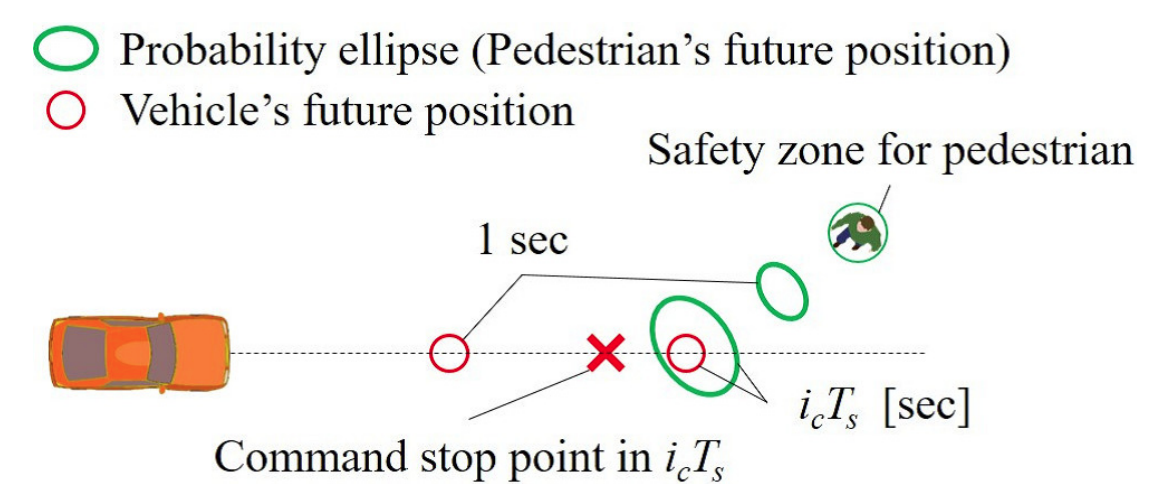
\includegraphics[width=8cm]{./fig/fig3.png}
    \caption{衝突検知の概要}
\end{figure}


\subsection{ブレーキコントロールシステム}
 モデル予測制御(MPC)は,車両を減速して$i_cT_s$の停止位置で停止するために使用される. MPCは,入力を最適化すると同時に,いくつかの制約を使用して各時点で将来の応答を予測する制御方法である.評価関数は次のとおり.
\begin{flalign}
    V[k]=\|\boldsymbol{Z}[k]-\boldsymbol{T}[k]\|_{Q}^{2}+\|\Delta \boldsymbol{U}[k]\|_{R}^{2}
\end{flalign}

なお

\begin{flalign}
    \mathbf{Z}[k]&=\left[\begin{array}{c}{z\left[k+H_{w} | k\right]} \\ {\vdots} \\ {\vdots} \\ {z\left[k+H_{p} | k\right]}\end{array}\right] \nonumber\\
    \boldsymbol{T}[k]&=\left[\begin{array}{c}{r\left[k+H_{w} | k\right]} \\ {\vdots} \\ {r\left[k+H_{p} | k\right]}\end{array}\right] \nonumber\\
    \boldsymbol{\Delta U}(k)&=\left[\begin{array}{c}{\Delta \hat{u}(k | k)} \\ {\vdots} \\ {\Delta \hat{u}\left(k+H_{u}-1 | k\right)}\end{array}\right] \nonumber
\end{flalign}

 $u$は制御範囲. QおよびRの説明は次のとおり.

\begin{flalign}
    \boldsymbol{Q}&=\left(\begin{array}{cccc}{\boldsymbol{Q}\left(H_{w}\right)} & {0} & {\cdots} & {0} \\ {0} & {\boldsymbol{Q}\left(H_{w}+1\right)} & {\cdots} & {0} \\ {\vdots} & {\vdots} & {\ddots} & {\vdots} \\ {0} & {0} & {\cdots} & {Q\left(H_{p}\right)}\end{array}\right) \nonumber\\
    \boldsymbol{R}&=\left(\begin{array}{cccc}{\boldsymbol{R}(0)} & {0} & {\cdots} & {0} \\ {0} & {\boldsymbol{R}(1)} & {\cdots} & {0} \\ {\vdots} & {\vdots} & {\ddots} & {\vdots} \\ {0} & {0} & {\cdots} & {\boldsymbol{R}\left(H_{u}-1\right)}\end{array}\right) \nonumber
\end{flalign}

 ここで,$H_w$は入力デッドタイムを示すウィンドウパラメーターである. $Q$と$R$は,それぞれ出力誤差と入力変化の重み行列である.式(17)の右側の第一項は司令値からの誤差を減らす効果があり,2番目の項は入力の突然の変化を抑制する. $r[k + i]$は次のように決定される.
\begin{flalign}
    \boldsymbol{r}[k+i]^{T}=\left(\begin{array}{lll}{x_{s}} & {y_{s}} & {0}\end{array}\right) \quad i_{c} \leq i \leq H_{p}
\end{flalign}


 式(18)は,$i_cT_s$ [sec]以降の車両位置を示す.ちなみに,出力と入力の変更と入力の制約は次のとおり.
\begin{flalign}
    \left|\hat{z}_{1}[k+i | k]-z_{1}[k | k]\right| \leq\left|x_{s}-z_{1}[k | k]\right| \\
    \left|\hat{z}_{2}[k+i | k]-z_{2}[k | k]\right| \leq\left|y_{s}-z_{2}[k | k]\right| \\
    |\Delta \hat{u}[k+i | k]| \leq \Delta u_{m a x} \\
    -\hat{\mu}_{\max } M g \leq u[k+i | k] \leq 0
\end{flalign}

 式(19)〜(20)は,コマンドの停止点を超えて実行されないための役割. (21)は,入力の変化がチューニングパラメーターである$\Delta u_{max}$より小さいことを示している. 式(22)は,タイヤの力を摩擦円理論で決定される最大制動力よりも小さくする. 式(19)〜(22)に示す制約の下,最適な入力変化$\Delta u[k | k]$が計算される. したがって,各車輪の最適な制動力は次のように決定される.
\begin{flalign}
    F_{d}^{c m d}=u[k-1]+\Delta u[k | k]
\end{flalign}

 MPCは,モデリングエラーを補正するためにフィードバックループが必要な開ループコントローラーである. したがって,MPCの内部でタイヤ力のフィードバックループを提供することが提案する. したがって,ブレーキ装置によって生成される基準トルクは次のように決定される.
\begin{flalign}
    T_{m}^{r e f}=\frac{K_{i}}{s}\left(F_{d}^{c m d}-\hat{F}_{d}\right)
\end{flalign}

 ここで,$K_i$および$\hat{F}_{d}$はそれぞれ,積分ゲイン,および駆動力オブザーバー(DFOB)によるタイヤ力の推定値を示す.

\subsection{オブザーバー設計}
 このセクションでは,タイヤの力と走行抵抗を推定する方法について説明する. タイヤの力を推定するために,駆動力オブザーバー(DFOB)が使用される. DFOBは,外乱トルクを正確に推定できる外乱オブザーバー(DOB)に基づいている. DFOBは次のように定式化される.
\begin{flalign}
    \hat{F}_{d}=\frac{1}{r_{w}}\left(\frac{g_{c u t}}{s+g_{c u t}}\left(T_{m}^{r e f}+g_{c u J} J \omega\right)-g_{c u t} J \omega\right)
\end{flalign}

 ここで,$g_{cut}$はローパスフィルター(LPF)のカットオフ周波数を示す. DFOBのブロック図を図4に示す. 制御性能を向上させるには,駆動抵抗$F_r$を推定する必要があり,式(26)を使用して推定できる. 走行抵抗推定器のブロック図を図5に示す.
\begin{flalign}
    \hat{F}_{r}=M \frac{g_{c u t}}{s+g_{c u t}} a-n \hat{F}_{d}
\end{flalign}

\begin{figure}[]
    \centering
    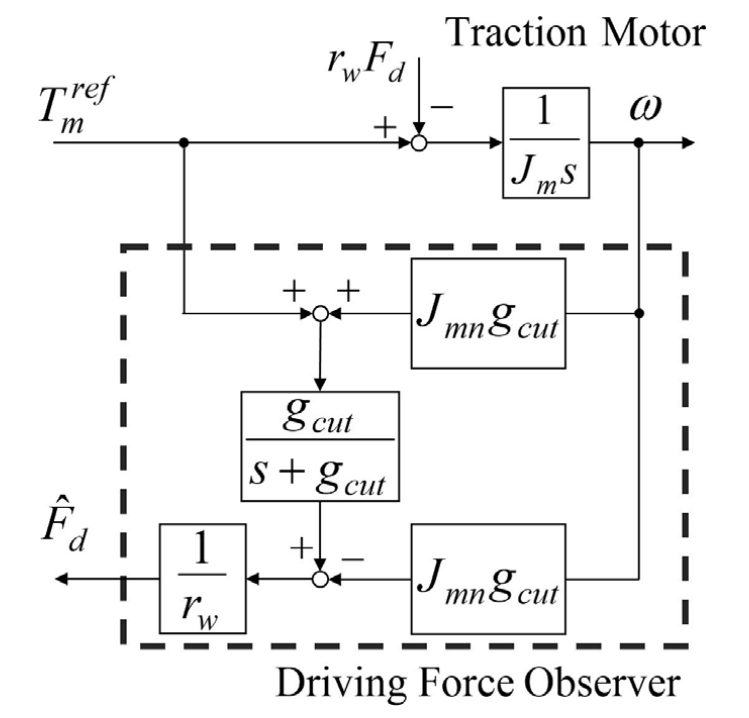
\includegraphics[width=8cm]{./fig/fig4.png}
    \caption{DFOBのブロック図}
\end{figure}
\begin{figure}[]
    \centering
    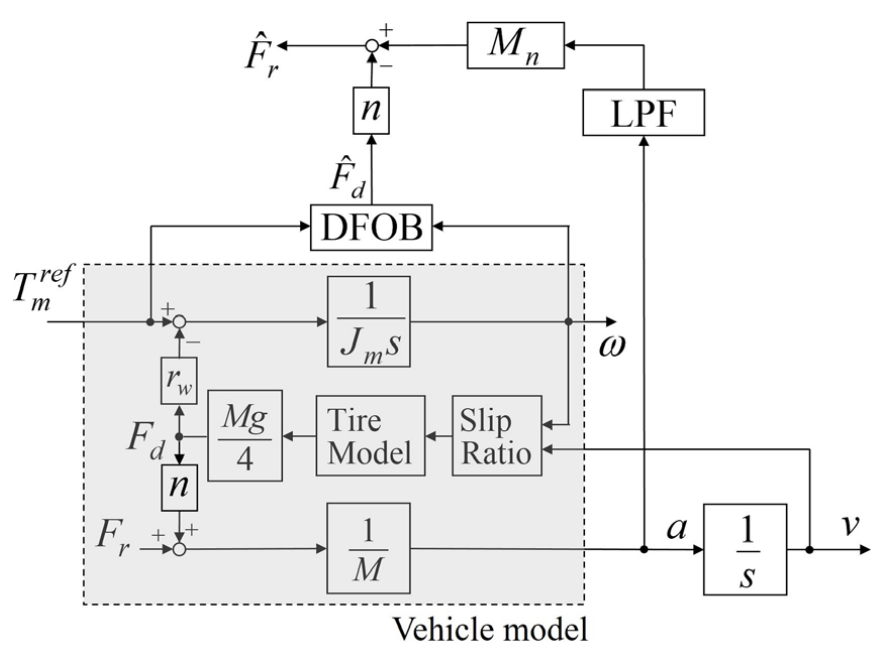
\includegraphics[width=8cm]{./fig/fig5.png}
    \caption{走行抵抗推定のブロック図}
\end{figure}

 aは車両の縦加速度. $\mu$は式(7)で推定でき,$\lambda$は式(8)で計算される. $lambda$と$\mu$を連続して取得して,最大摩擦係数$μ_{max}$は,最小二乗法(LSM)を使用して$\mu-\lambda$曲線を2次関数に近似することによって推定され,式のMPCの制約として$\mu_{max}$を設定する.
 最後に,ブレーキシステム全体を図6に示す.
\begin{figure}[]
    \centering
    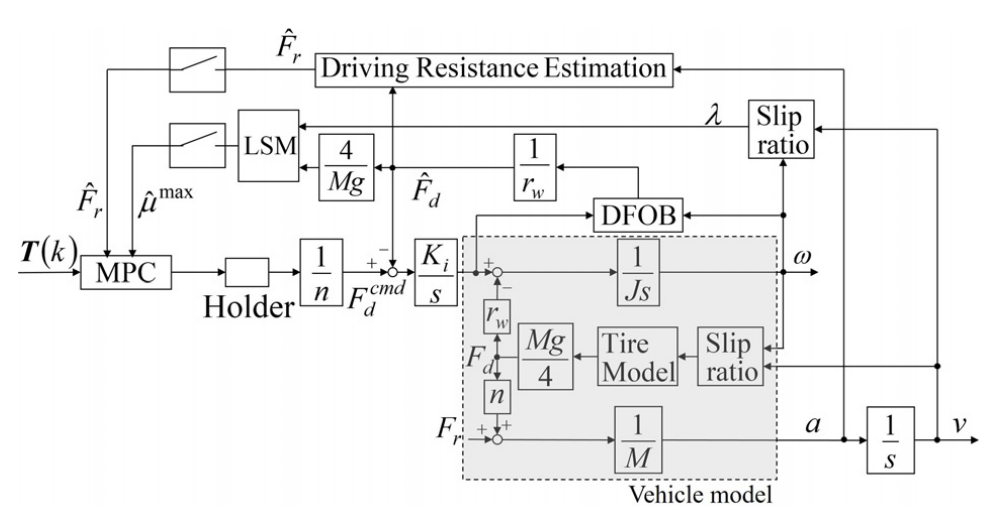
\includegraphics[width=8cm]{./fig/fig6.png}
    \caption{ブレーキシステム全体のブロック図}
\end{figure}


\section{シミュレーション}
\subsection{シミュレーション環境}
 このシミュレーションでは,路面を再現するマジックフォーミュラタイヤモデルを使用した. 駆動抵抗は,転がり抵抗,空気抵抗,勾配抵抗で構成される. 各力は式 (27)〜(30)で定式化される.
\begin{flalign}
    F_{\text {roll}}&=-C_{r r} M g \\
    F_{\text {air}}&=-\frac{1}{2} \rho C_{D} S v^{2} \\
    F_{\text {grad}}&=M g \sin \theta_{\text {grad}} \\
    F_{r}&=F_{\text {roll}}+F_{\text {air}}+F_{\text {grad}}
\end{flalign}

\begin{figure}[]
    \centering
    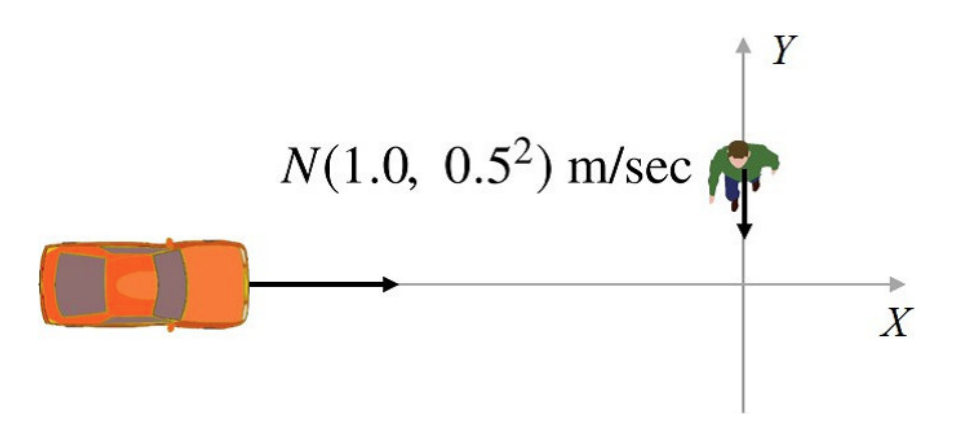
\includegraphics[width=8cm]{./fig/fig7.png}
    \caption{シミュレーションの状況}
\end{figure}

\begin{table}[]
    \centering
    \caption{シミュレーションでの道路環境}
    \begin{tabular}{|c|c|c|}
    \hline
    Road & Surface & Gradient \\ \hline
    1    & Dry     & Downhill \\ \hline
    2    & Wet     & Flat     \\ \hline
    \end{tabular}
\end{table}

\begin{table}[htbp]
    \centering
    \caption{シミュレーション条件}
    \scalebox{0.87} {
        \begin{tabular}{|c|c|c|}
            \hline
            Parameter                                  & Value   & Unit     \\ \hline
            Vehicle mass $M$                           & 1000    & kg       \\ \hline
            Wheel radius $r_{\omega}$                  & 0.302   & m        \\ \hline
            Number of controlled wheels $n$            & 4       &          \\ \hline
            Motor Inertia $J_{\omega h}$               & 1.24    & kgm$^2$  \\ \hline
            Motor viscosity coefficient $D_{\omega h}$ & 0.00040 & Nsec/m   \\ \hline
            Motor coulomb friction $f_{\omega h}$      & 0.001   &          \\ \hline
            Sample time in MPC $T_s$                   & 0.1     & sec      \\ \hline
            Integral gain $K_i$                        & 50000   &          \\ \hline
            prediction horizon $H_p$                   & 30      &          \\ \hline
            Control horizon $H_u$                      & 10      &          \\ \hline
            Safety zone for pedestrian $R_h$           & 0.5     &          \\ \hline
            Downhill gradient $\theta_p$               & 5       & deg      \\ \hline
            Rolling resistance coefficient $C_{rr}$    & 0.01    &          \\ \hline
            Air resistance coefficient $C_d$           & 0.3     &          \\ \hline
            Projected area $S$                         & 1.754   & m$^2$    \\ \hline
            Air density $\rho$                         & 1.225   & kg/m$^3$ \\ \hline
        \end{tabular}
    }
\end{table}

 シミュレーションパラメータを表3に示す.シミュレーション1では,道路環境1での走行時に走行抵抗が補正されるかどうかの比較を行う.さらに,道路環境2では路面での最大摩擦係数の推定の有無について比較を行う.

\subsection{シミュレーション結果}
 シミュレーション1の結果を図8と〜図10に示す.図8は,車両と歩行者の位置を示している. 図8によると,システムは良好に機能し,車両は運転抵抗を補償することで歩行者の前方に停止した. 走行抵抗補正がない場合,車両は歩行者の前で停止できなかった. したがって,駆動抵抗を補償することが検証された.\\
 また,図9は,推定値と駆動抵抗の真値との比較を示しており,値が真値に近づいたことを示している.図10から提案手法で適切な制動力が発生していることを確認できる.補償付き制御法を利用する場合は,駆動力を考慮した制動力を車両に追加する.道路環境1は下り坂であり,走行抵抗には正の勾配抵抗が含まれる.したがって,司令位置で停止するには,車両を強くブレーキする必要がある.\\
 同様に,シミュレーション2の結果を図11〜図13に示す.\\
 図11は,車両と歩行者の位置を示している.図11によれば,路面が濡れていても最大摩擦係数を推定することにより,車両は歩行者の前方を停止した.図12は最大摩擦係数の推定結果を示しており,推定値が真の値よりわずかに小さい値に収束したことを示している.図10から提案手法で適切な制動力が発生することが確認された.最大摩擦係数を推定しない場合,タイヤ力の絶対値は2.4秒から減少した.これは,制動力が摩擦円理論の制限を超え,タイヤがスリップしたことを示している.したがって,推定最大摩擦係数に対する有効性が確認された.
\newpage

\begin{figure}[H]
    \centering
    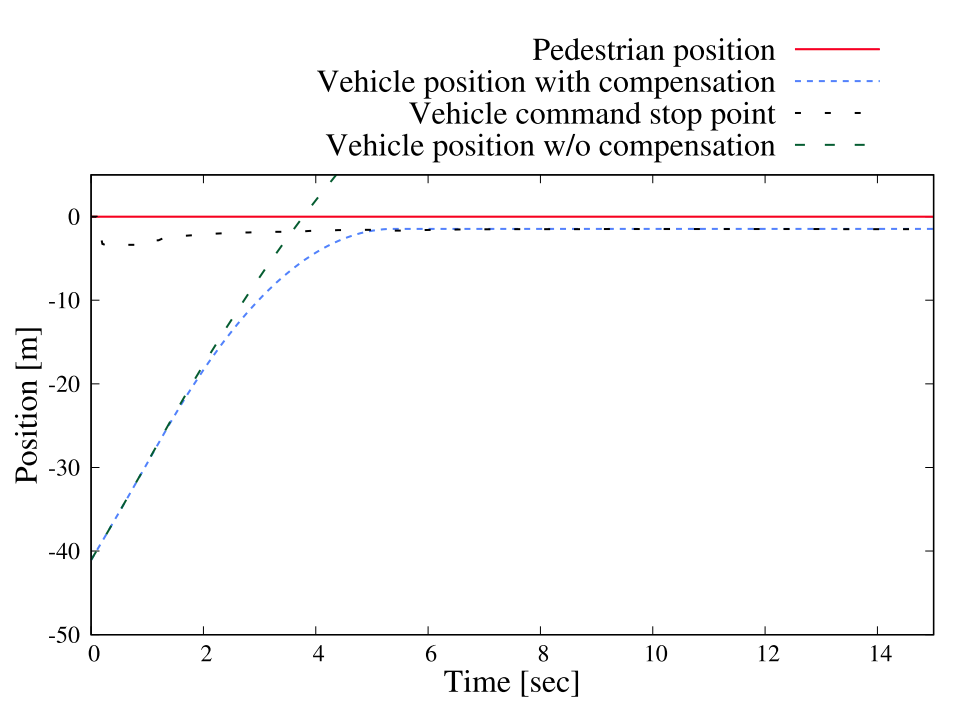
\includegraphics[width=8cm]{./fig/fig8.png}
    \caption{車両位置のシミュレーション1結果}
\end{figure}

\begin{figure}[H]
    \centering
    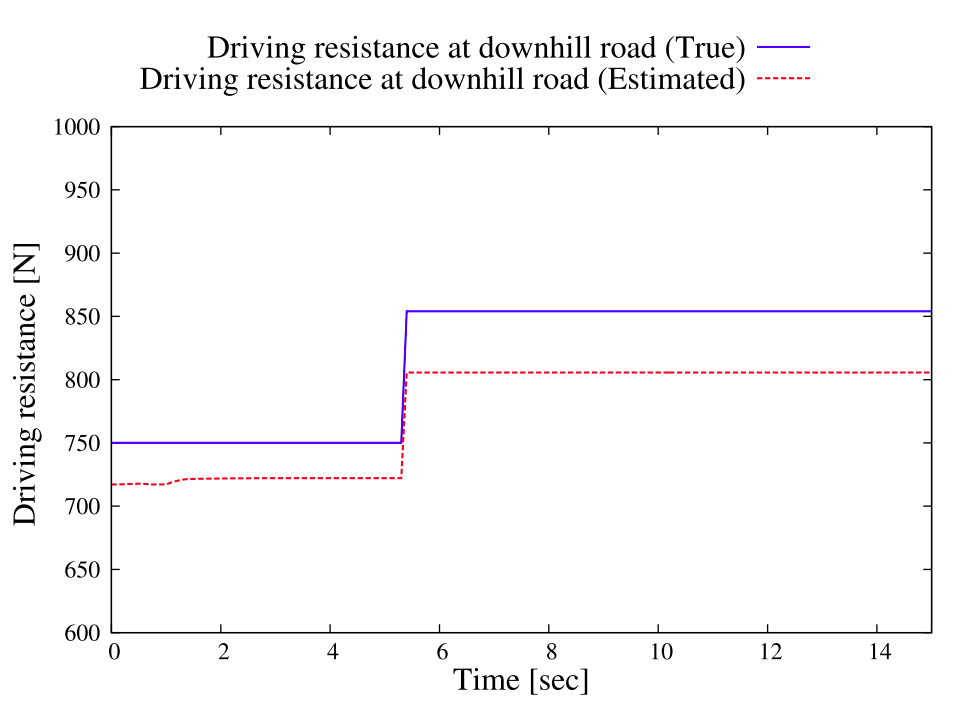
\includegraphics[width=8cm]{./fig/fig9.png}
    \caption{運転抵抗のシミュレーション1結果}
\end{figure}

\begin{figure}[H]
    \centering
    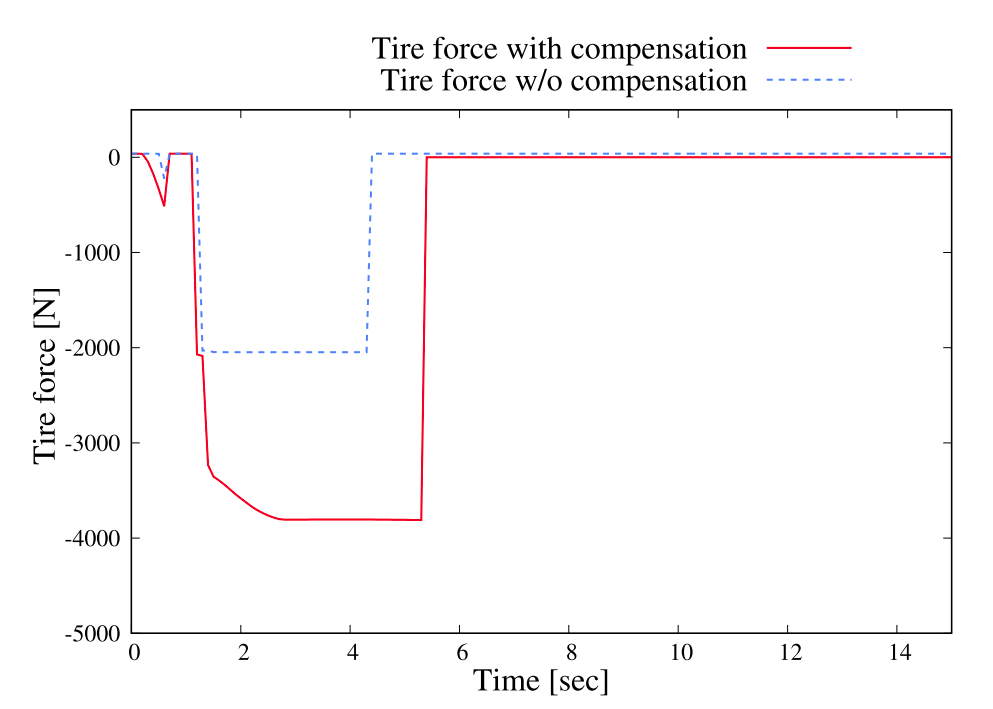
\includegraphics[width=8cm]{./fig/fig10.png}
    \caption{タイヤ力のシミュレーション1結果}
\end{figure}
\newpage
\begin{figure}[H]
    \centering
    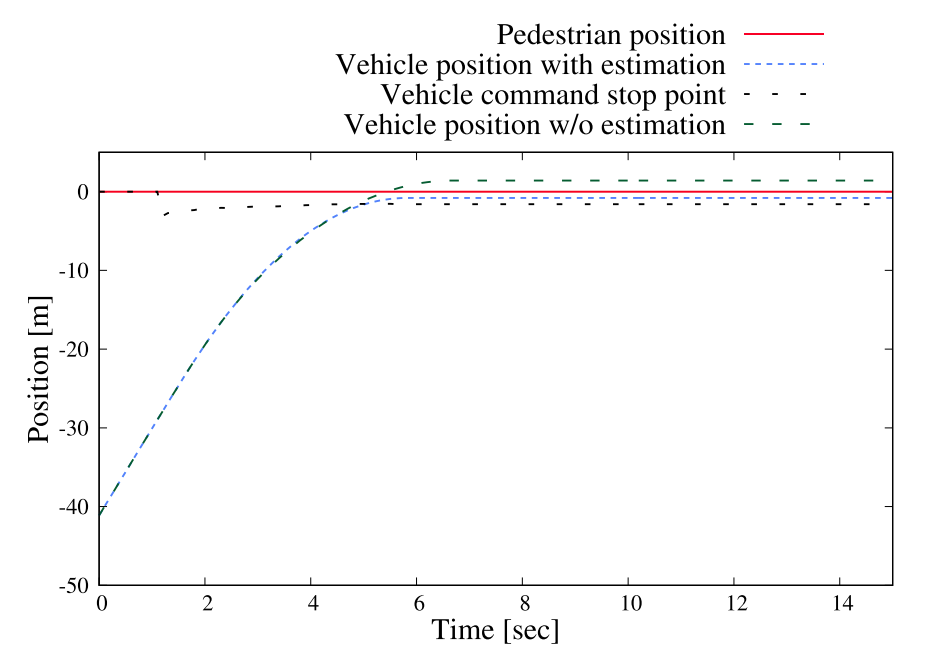
\includegraphics[width=8cm]{./fig/fig11.png}
    \caption{車両位置のシミュレーション2結果}
\end{figure}

\begin{figure}[H]
    \centering
    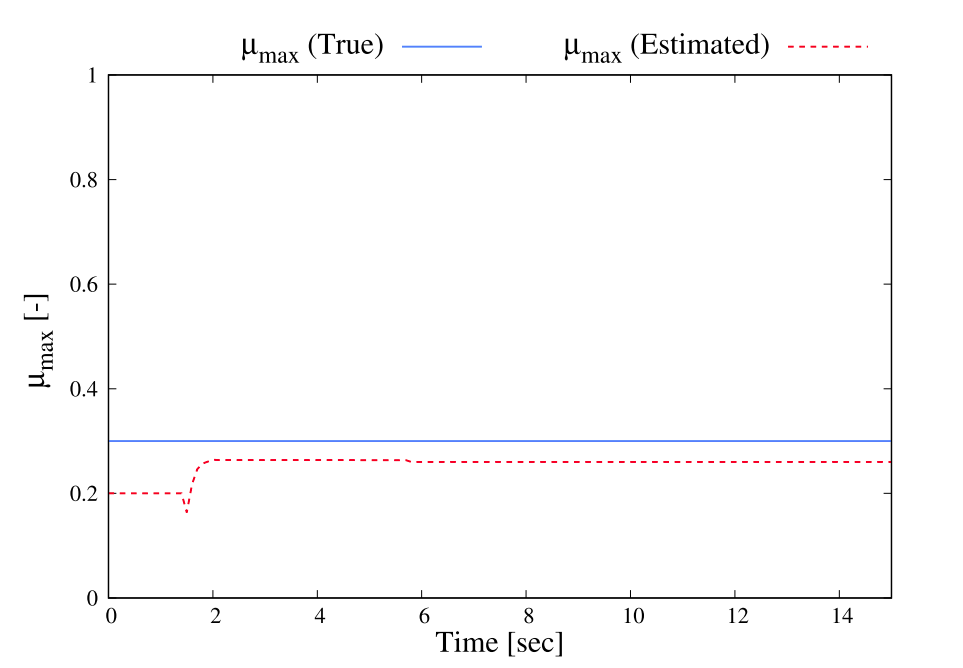
\includegraphics[width=8cm]{./fig/fig12.png}
    \caption{運転抵抗のシミュレーション2結果}
\end{figure}

\begin{figure}[H]
    \centering
    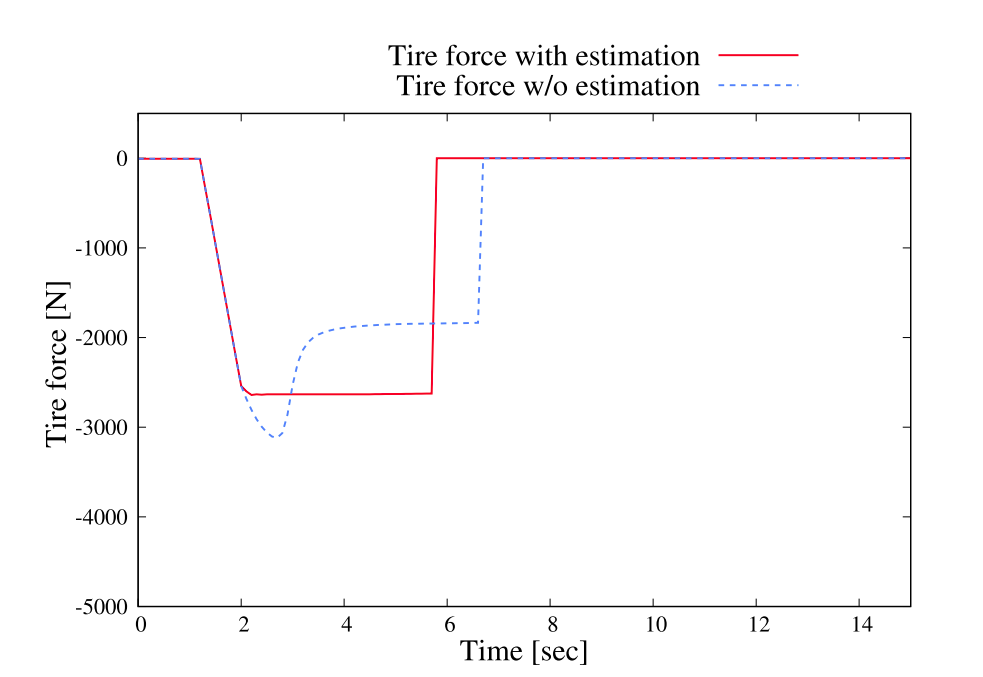
\includegraphics[width=8cm]{./fig/fig13.png}
    \caption{タイヤ力のシミュレーション2結果}
\end{figure}

\newpage
\newpage

\section{実験}
 実験は,提案された方法の有効性を確保するために実施した. 実験では,図14に示すように,ZMP Inc.が作成した1:10スケールの車両モデルであるRoboCar 1/10を使用した.このモデルには速度コントローラーが含まれ,車両システムの入力は速度のみである. そのため,MPCから取得した速度値を入力に使用し,駆動力フィードバックの代わりに車両速度フィードバックを実装した. 実験のブロック図を図15に示す.表4で実験のセットアップを示す.
\begin{figure}[H]
    \centering
    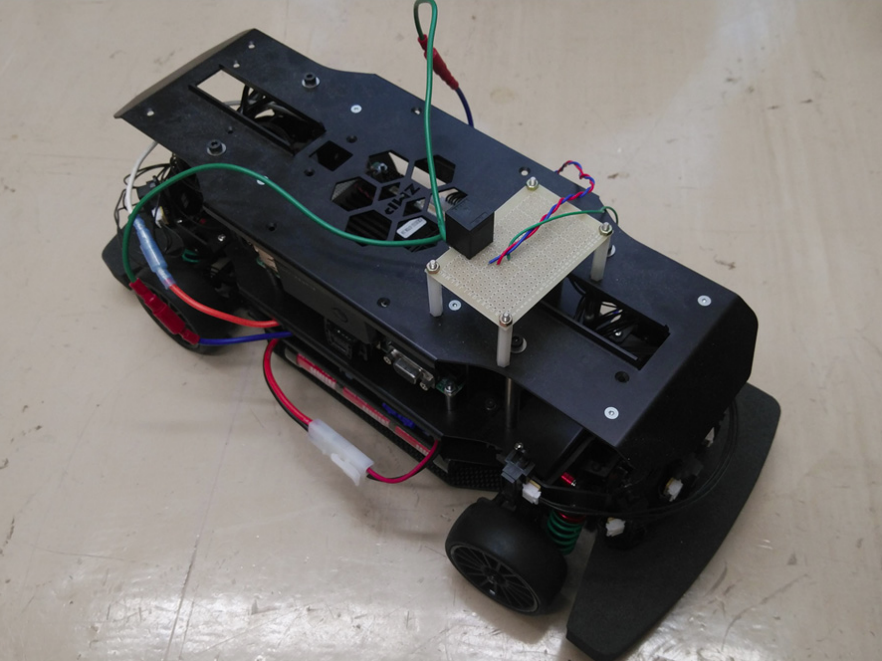
\includegraphics[width=8cm]{./fig/fig14.png}
    \caption{実験車両}
\end{figure}
\begin{figure}[H]
    \centering
    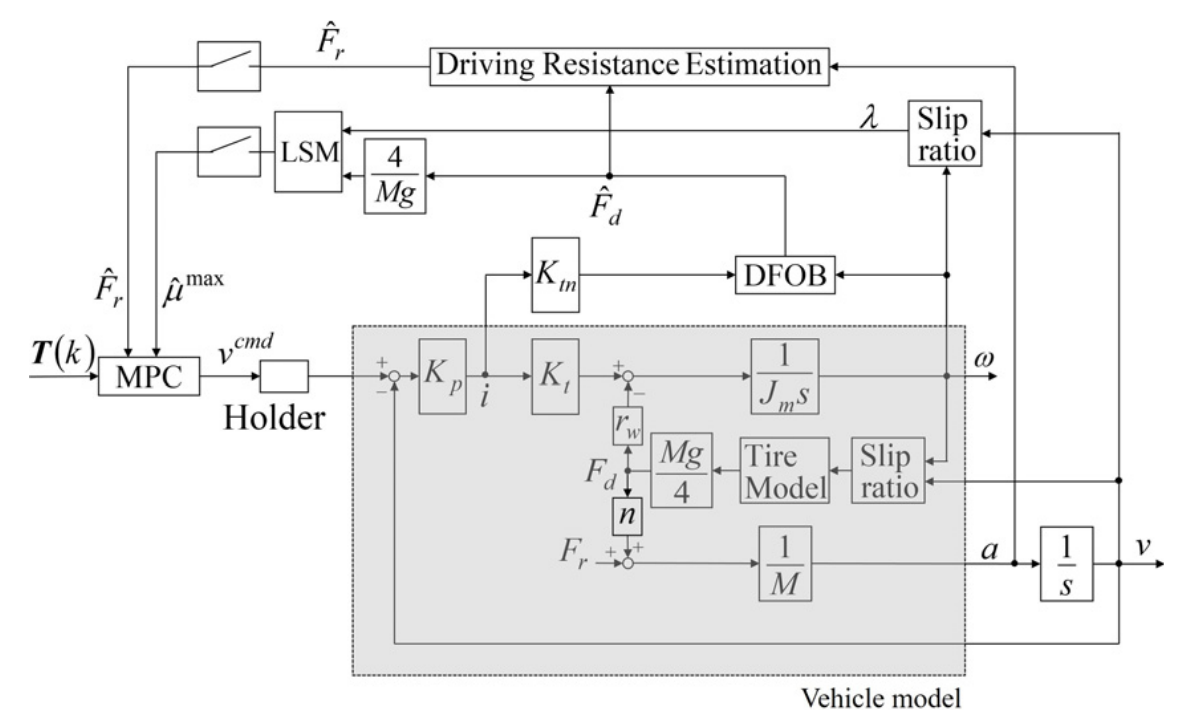
\includegraphics[width=8cm]{./fig/fig15.png}
    \caption{実験のブロック図}
\end{figure}

\begin{table}[htbp]
    \centering
    \caption{実験のパラメータ}
    \scalebox{0.81} {
        \begin{tabular}{|c|c|c|}
            \hline
            Parameter                                 & Value        & Unit      \\ \hline
            Vehicle mass $M$                          & 2.9          & kg        \\ \hline
            Number of controlled wheels $n$           & 2            &           \\ \hline
            Sample time in MPC $T_s$                  & 0.1          & sec       \\ \hline
            Proportional gain $K_p$                   & 50           &           \\ \hline
            prediction horizon $H_p$                  & 30           &           \\ \hline
            Control horizon $H_u$                     & 10           &           \\ \hline
            Safety zone of pedestrian $R_h$           & 0.05         & m         \\ \hline
            Torque coeffcient $K_t$                   & 0.002354     &           \\ \hline
            Motor inertia $J_n$                       & 4.342 x 10 6 & kgm$^2$   \\ \hline
            Motor viscosity coeffcient $D_{\omega h}$ & 9.416 x 10-7 & Nmsec/rad \\ \hline
            Motor coulomb friction $f_{\omega h}$     & 2.532 x 10-3 & Nm        \\ \hline
        \end{tabular}
    }
\end{table}


\begin{figure}[H]
    \centering
    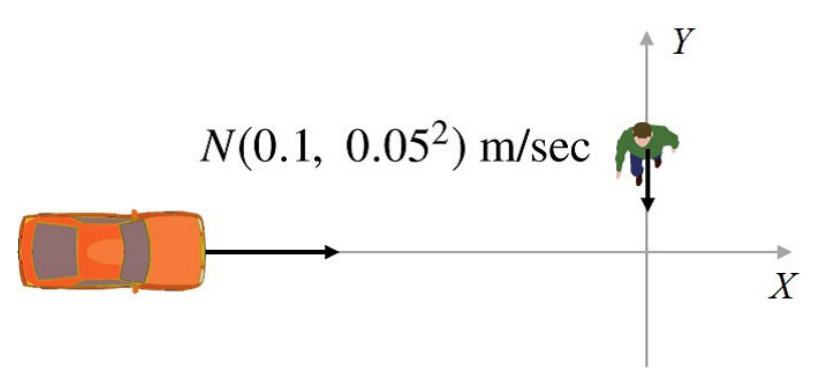
\includegraphics[width=8cm]{./fig/fig16.png}
    \caption{実験の状況}
\end{figure}

実験手順は次のとおり.
\begin{enumerate}
    \item PCで仮想歩行者の位置を生成
    \item PCが情報を車両に送信
    \item 車両は歩行者の位置を受け取り,制御を実行
\end{enumerate}

歩行者の位置は,図16に従ってPCによって計算された.

実験結果を図17,18に示す.図17は,車両と歩行者の位置を示している. 車両は歩行者の前の指令停止地点近くで停止した. それは,提案した方法が衝突回避システムとして非常にうまく機能することを示した. 図18によれば,走行抵抗推定器は定常値に収束する. ただし,シミュレーション結果と比較して,駆動抵抗は駆動力よりもはるかに大きかった. この現象は,転がり抵抗が大きいタイヤが原因で発生したため,制動力を適切に制御して,車両を指令停止点で停止させる必要がある. 補償なしのブレーキシステムの場合,ブレーキ力は変動した. その理由は,MPCが外乱と車両の状態を正確に予測できなかったため,運転抵抗がシステムに影響を与えたためである. 以上より,提案手法の有効性は実験により確認された.
\begin{figure}[H]
    \centering
    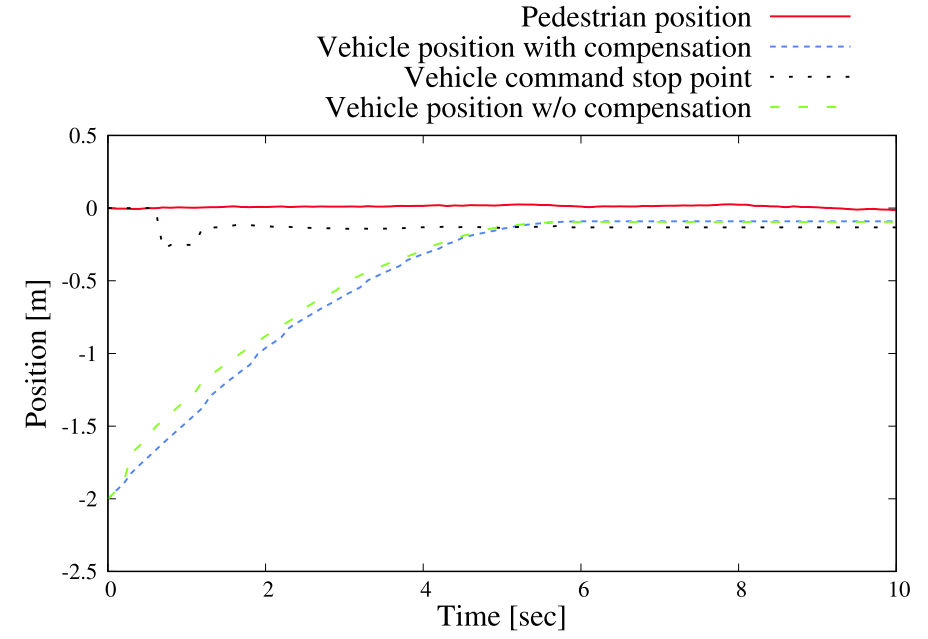
\includegraphics[width=8cm]{./fig/fig17.png}
    \caption{車両位置の実験結果}
\end{figure}
\begin{figure}[H]
    \centering
    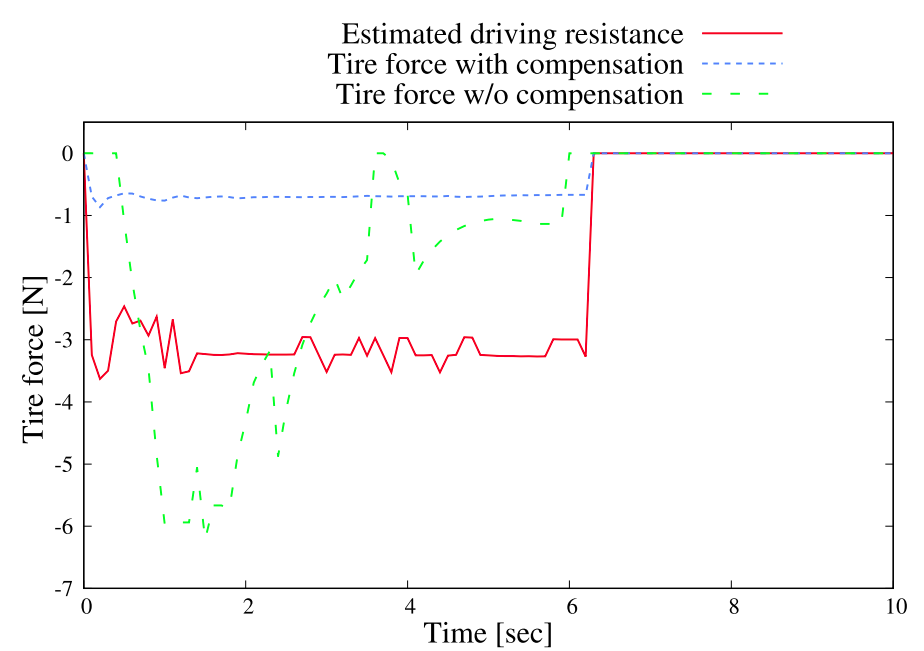
\includegraphics[width=8cm]{./fig/fig18.png}
    \caption{タイヤ力の実験結果}
\end{figure}

\section{結論}
 本稿の目的は,歩行者との衝突を回避するために,自動減速システムを実現することである.提案システムは,現在の位置から歩行者の将来の位置を予測し,衝突確率を検出することが可能である.また,走行抵抗とモデル化誤差を補償することができるMPCとコントローラを,この論文で提案されている.\\
 まず,歩行者の速度は,カルマンフィルターにより,現在の歩行者の位置から推定される.将来の歩行者の予想位置は,歩行者の速度から予測され,制動力の指令値は,MPCによって計算される.ここでは,MPCは外乱とパラメータ誤差の影響を強く受けるため,制御性能を向上させるために,制動力のフィードバックループが提案されている.さらに,提案されたシステムには,走行抵抗の推定量が含まれている.これにより,歩行者の将来の位置を予測し,衝突の危険性を検出することが可能である.さらに,駆動抵抗を補償し,制動力を制御することにより,外乱感度を低減しながらシステムの追従性を向上させることができる.\\
 提案手法の有効性は,シミュレーションと実験により検証されている.このシステムを活用して,事故の数を減らすことが期待される.

\end{document}
